\documentclass[12pt]{article}
\usepackage{amsmath}
\usepackage{amssymb}
\usepackage{amsthm}
\usepackage{graphicx}
\usepackage{algorithm}
\usepackage[noend]{algpseudocode}
\usepackage{cite}
\newtheorem{lemma}{Lemma}

\begin{document}
\title{Solving Avalanche's Multi-Coloring Problem via Ordering Constraint Graphs}
\author{John Boyd\thanks{john@coldnoise.net}}
\date{November 22, 2024}
\maketitle

\begin{abstract}
Avalanche consensus achieves Byzantine agreement with constant-sized
communication, enabling horizontal scaling to large validator sets. However,
the protocol suffers from a multi-coloring problem: when conflict sets contain
more than two choices, convergence probability decreases toward zero as choices
increase. Existing solutions either sequentialize consensus or restrict
transaction production, creating a trade-off between performance and
decentralization. This work presents a novel solution by extracting pairwise
ordering constraints from transactions to construct a constraint DAG, then
executing Avalanche to reach agreement on the constraint graph rather than the
transaction graph. By extracting only pairwise constraints — specifically,
ordering relationships between pairs of parent transactions — we ensure each
constraint conflicts with at most one other constraint (its opposite),
guaranteeing multi-colored conflict sets cannot arise. Avalanche consensus
therefore converges on the constraint DAG. Once peers agree on the ordering
constraints, they deterministically derive total transaction ordering without
additional communication. This approach preserves Avalanche's $O(1)$
convergence time while maintaining full decentralization, at the cost of
$O(n^2)$ communication overhead per transaction, where $n$ is the number of
parent transactions. Consequently, peers also reach agreement on total
transaction ordering, a property not provided by Avalanche, enabling support
for any general replicated state machine.
\end{abstract}

\section{Introduction}
The Avalanche consensus protocol \cite{rocket} is unique in its ability to
reach Byzantine agreement with only constant-sized communication. This allows
horizontal scaling without network partitioning—new validators may join to
increase security and availability without degrading performance.

However, Avalanche suffers from a fundamental limitation known as the
multi-coloring problem. When transactions form conflict sets with more than two
options, the probability of convergence decreases as the number of
options increases, potentially leading to liveness failures.

The Snowman consensus protocol addresses the multi-coloring problem through
binary decomposition \cite{buchwald2024frosty}, but this requires executing
multiple sequential instances of Avalanche consensus, hindering performance.
The Snowman authors suggest the use of elected proposers to avoid multi-colored
conflicts, reducing the probability of conflicts to mitigate this performance
penalty.

This work proposes a novel solution to the multi-coloring problem that
eliminates the need for sequential Avalanche instances while preserving the DAG
structure and $O(1)$ convergence time, trading increased bandwidth for faster
concurrent convergence. The key insight is to deliberately extract
only pairwise ordering constraints from transactions to form a constraint DAG.
By restricting constraints to pairs of transactions, we ensure each constraint
$[a,b]$ conflicts only with $[b,a]$, making all conflict sets binary. Avalanche
consensus is therefore guaranteed to converge on the constraint DAG. Once peers
agree on the preferred constraints, they can deterministically compute the
total transaction ordering.

An additional benefit of this construction is that peers achieve agreement on
total transaction ordering, a property not provided by standard Avalanche. This
enables the protocol to support general replicated state machines and other
applications requiring transaction sequencing.

\section{Background}
\subsection{Avalanche Consensus}
Avalanche is a probabilistic, leaderless consensus protocol that uses network
sampling to create a metastable mechanism driving participants to converge on
decisions \cite{rocket}. The protocol records transactions into a DAG. As
transactions disseminate, nodes insert them into the DAG and group them into
conflict sets. Each node queries a randomly selected, constant-sized subset of
peers for their preferred transaction in each conflict set. Preferred
transactions receive chits and accumulate confidence scores. Once a transaction
reaches the confidence threshold, it is considered final.

A node's preference may change if subsequent queries indicate a transaction is
no longer connected to the most preferred graph. This rule to adopt peer
preferences makes indecision metastable and drives convergence.

While Avalanche provides agreement on which transactions are accepted, it does
not provide agreement on the ordering of those transactions. Because
transactions may be inserted simultaneously into the DAG, different peers may
observe transactions in different orders, and Avalanche provides no mechanism
to reconcile these differences.

\subsection{The Multi-Coloring Problem}
\label{sec:multicolor}
Avalanche consensus can be modeled as a graph coloring process over transaction
conflict sets. Each conflict set is a vertex, and peers assign colors
representing preferred transactions. Consensus is achieved when all peers agree
on each vertex's color.

The multi-coloring problem arises when conflict sets have more than two
options. As described in \cite{buchwald2024frosty}, convergence probability
decreases as the probability of two peers initially assigning the same color
decreases. Assuming uniform random color assignment, convergence probability
approaches zero as the number of colors increases.

For two-colored graphs, disagreement is metastable. The sampling process makes
progress in expectation and eventually converges. This is not true for
multi-colored graphs, posing a fundamental challenge to applications whose
transactions do not form binary conflict sets.

\subsection{Snowman's Approach}
Snowman consensus solves the multi-coloring problem through binary
decomposition \cite{buchwald2024frosty}. Each multi-colored conflict set of
size $L$ is decomposed into $\log_2(L)$ two-colored subsets. Snowman
sequentially executes Avalanche consensus on each subset, and because each is
binary, convergence is guaranteed. The preferences form a path to exactly one
transaction in the original conflict set.

While Snowman guarantees convergence, it increases convergence time by requiring
multiple sequential Avalanche processes. To mitigate this, the authors suggest
a proposer election process to reduce the probability of conflicts.
Importantly, this conflicts with one of Avalanche's defining properties:
leaderless consensus. Concretely, this trade-off compromises decentralization to
achieve performance.

\section{Ordering Constraint Graphs}
\subsection{Core Idea}
We solve the multi-coloring problem by extracting pairwise ordering constraints
from transactions to form a constraint DAG. The critical design decision is to
extract only binary constraints—specifically, ordering relationships between
pairs of parent transactions. This is conceptually similar to the binary set
decomposition of \cite{buchwald2024frosty}; however, the use of ordering
constraints allows us to create a constraint graph and make progress on each
constraint concurrently, as opposed to sequentially. Intuitively, these partial
ordering constraints directly relate to the underlying source of conflicts in
the set (disagreement about order of observation).

This design ensures that each constraint $[p_0, p_1]$ conflicts only with its
opposite $[p_1, p_0]$, making the maximum conflict set size exactly 2.
Therefore, Avalanche consensus is guaranteed to converge on the constraint DAG.
Since the constraint graph fully describes the transaction graph, by extension
we also reach agreement on the transaction graph.

\textbf{Trade-off:} A transaction with $n$ parents generates $\binom{n}{2} + n
= O(n^2)$ constraints, each requiring Avalanche consensus. This increases
communication overhead compared to standard Avalanche's single consensus
instance per transaction. However, these constraint instances execute
concurrently rather than sequentially, preserving $O(1)$ convergence time in
rounds while accepting higher bandwidth utilization. For applications where $n$
is bounded by a small constant, this overhead is acceptable.

Multiple Avalanche instances must execute for a given transaction, but
crucially they execute \emph{concurrently} rather than sequentially. This
allows convergence in the same time as standard Avalanche consensus, at the
cost of increased communication compared to basic Avalanche, but with
significantly faster convergence than Snowman.

\subsection{Notation}
We use two DAGs: the \emph{transaction DAG} whose vertices are transactions,
and the \emph{constraint DAG} whose vertices are ordering constraints.
Transactions are annotated by height $h$ and observation order $i$ as
$t_{h,i}$. For example, $t_{9,0}$ denotes the first transaction observed at
height 9.

Ordering constraints are denoted $[t_a, t_b]$, where $t_a$ is constrained to
precede $t_b$. Constraints may be referenced as $c_{h,i,n}$, the $n^{\text{th}}$
constraint of transaction $t_{h,i}$.

A special case exists for single-parent transactions: the \emph{empty
constraint} $[t_a, -]$. This does not actually constrain $t_a$'s ordering; it
exists only to assist constraint DAG connectivity.

\subsection{Constructing the Constraint DAG}
Each transaction commits to a list of parent transactions which precede it, in
the order in which they were observed by the node that produced this
transaction. Ordering constraints are determined by transforming the
transaction's list of parents into a list of ordered pairs. A transaction
commits to:
\begin{enumerate}
\item The empty constraint for each parent
\item A pairwise ordering constraint for every ordered pair of parents consistent with the transaction's stated parent sequence
\end{enumerate}

For example, transaction $t_{h,i}$ with parents $p_0, p_1, p_2$ (in that order)
commits to: $[p_0, -]$, $[p_1, -]$, $[p_2, -]$, $[p_0, p_1]$, $[p_0, p_2]$,
$[p_1, p_2]$. Each constraint implicitly depends on the parent transactions it
references. These dependencies form the edges of the constraint DAG.

\begin{figure}
  \centering
  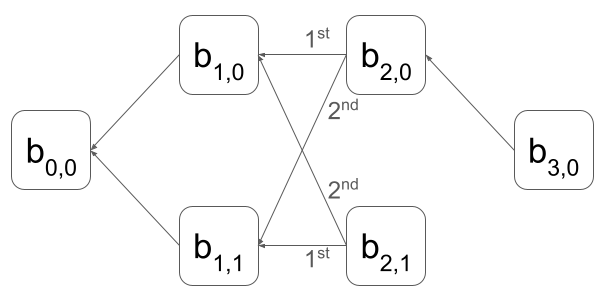
\includegraphics[width=\columnwidth]{images/block_dag.png}
  \caption{Example transaction DAG. Transactions $b_{2,0}$ and $b_{2,1}$ conflict due to their opposing parent orderings—they both reference $b_{1,0}$ and $b_{1,1}$ but in opposite order.}\label{fig:transaction_dag}
\end{figure}

\begin{figure}
  \centering
  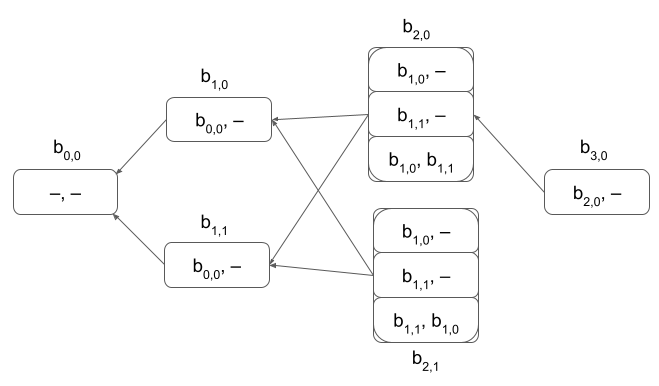
\includegraphics[width=\columnwidth]{images/block_dag_with_constraints.png}
  \caption{Expanded view showing parent ordering constraints for each transaction in Figure \ref{fig:transaction_dag}. Note that each constraint expresses an ordering relationship between exactly two parents.}\label{fig:transaction_dag_with_constraints}
\end{figure}

\subsection{Conflict Sets in the Constraint DAG}
To apply Avalanche consensus to the constraint DAG, we must define conflict
sets. Two constraints $[a, b]$ and $[c, d]$ conflict if and only if $a = d$ and
$b = c$. Because we extract only pairwise constraints, each constraint
conflicts with at most one other constraint—its opposite. Constraints with no
conflicts form singleton conflict sets.

Figure \ref{fig:constraint_dag} illustrates the constraint DAG for our example.
Constraints $[b_{1,0}, b_{1,1}]$ and $[b_{1,1}, b_{1,0}]$ are in the same
conflict set because they reference parent transactions in opposing order.
Avalanche consensus resolves the preferred constraint in each conflict set.

\begin{figure}
  \centering
  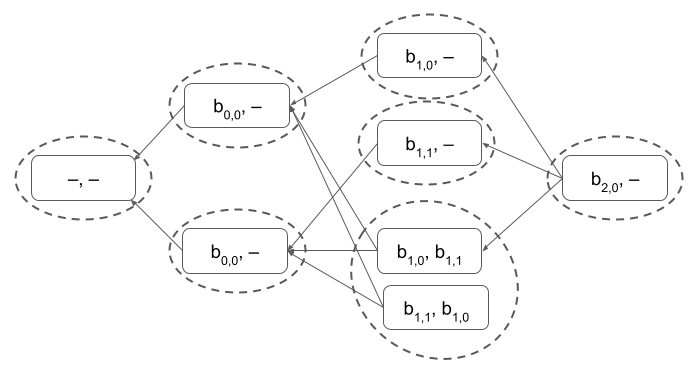
\includegraphics[width=\columnwidth]{images/constraint_dag.png}
  \caption{Constraint DAG constructed from transactions in Figure \ref{fig:transaction_dag_with_constraints}. Conflict sets are indicated by dashed lines. Each conflict set contains at most two constraints.}\label{fig:constraint_dag}
\end{figure}

Consensus is reached by executing Avalanche on constraint conflict sets. Once
every constraint committed by a transaction is accepted into the constraint
DAG, that transaction is inferred to be accepted into the transaction DAG
without any additional consensus process.

\subsection{Handling Incompatible Constraints}
\label{sec:incompatible}
An important property of this construction is that incompatible constraints can
temporarily coexist in the constraint DAG during consensus. Consider the
following scenario:
\begin{itemize}
\item Transaction $A$ commits to constraint $[p_1, p_2]$
\item Transaction $B$ commits to constraint $[p_2, p_3]$
\item Transaction $C$ commits to constraint $[p_3, p_1]$
\end{itemize}

While these constraints are pairwise non-conflicting (none are direct
opposites), they are mutually \emph{incompatible}—they cannot all be satisfied
in any valid total ordering. However, this does not create a structural problem
for the protocol:

Any future transaction that attempts to build upon all three incompatible
constraints will necessarily create a \emph{direct conflict} with at least one
of them. To extend the DAG beyond these three transactions, a new
transaction must specify an ordering over some subset of $\{p_1, p_2, p_3\}$.
Any such ordering will agree with at most two of the three incompatible
constraints and will conflict with the third.

As new transactions are proposed and Avalanche consensus executes on their
constraints, the metastability of indecision drives the network toward
preferring transactions (and their constraints) that form a consistent
ordering. The incompatible constraint that receives less support through this
process will eventually be rejected, causing its parent transaction to be
rejected as well.

This behavior is analogous to standard Avalanche: multiple conflicting
transactions can temporarily exist in the DAG, but as the network builds upon
preferred transactions, non-preferred transactions become disconnected from the
preferred frontier and are eventually rejected.

Therefore, temporary coexistence of incompatible constraints does not threaten
correctness or liveness. The protocol naturally resolves these
incompatibilities through the standard Avalanche consensus mechanism.

\subsection{Determining Transaction Sequence}
As constraints are accepted, we can compute the final sequence of transactions.
Once every constraint referencing any transaction in the progeny of transaction
$t$ is accepted, the sequence leading to $t$ is computed recursively: merge the
sequences at each parent (eliminating duplicates), then append each parent in
order, as shown in Algorithm \ref{alg:sequencing}.

\begin{figure}
\begin{algorithmic}[1]
    \Procedure{sequenceAt}{$t$}
      \State $\mathcal{S} := \emptyset$
      \For{$t' \in \mathcal{T}: t' \stackrel{*}{\gets} t$}
        \For{$t'' \in \mathcal{T}: t'' \in \Call{sequenceAt}{t'} \land t'' \notin \mathcal{S}$}
          \State $\mathcal{S} = \mathcal{S} \,||\, t''$
        \EndFor
      \EndFor
      \For{$t' \in \mathcal{T}: t' \stackrel{*}{\gets} t$}
          \State $\mathcal{S} = \mathcal{S} \,||\, t'$
      \EndFor
      \State \Return $\mathcal{S}$
    \EndProcedure
\end{algorithmic}
\caption{Algorithm to determine the sequence of transactions preceding a given transaction.} \label{alg:sequencing}
\end{figure}

When two transactions disagree on parent ordering, they produce conflicting
pairwise constraints. Eventually one constraint is rejected from the constraint
DAG, at which point its transaction is rejected from the transaction DAG. This
ensures the transaction graph can never disagree with the constraint graph.

Applying this algorithm to Figure \ref{fig:transaction_dag} to determine the
sequence at $b_{3,0}$, we obtain: $b_{0,0}$, $b_{1,0}$, $b_{1,1}$, $b_{2,0}$,
$b_{3,0}$.

\section{Analysis}
Table \ref{tab:comparison} provides an overview of the comparison of this work
with Avalanche consensus and Snowman.

\begin{table}[h]
\centering
\begin{tabular}{|l|c|c|c|}
\hline
\textbf{Property} & \textbf{This Work} & \textbf{Avalanche \cite{rocket}} & \textbf{Snowman \cite{buchwald2024frosty}} \\
\hline
Liveness & Guaranteed & Fails with & Guaranteed \\
 & & multi-coloring & \\
\hline
Time to & $O(1)$ & $O(1)$ & $O(\log L)$ \\
Convergence & & (no multi-color) & \\
\hline
Communication & $O(n^2)$ per & $O(1)$ per & $O(\log L)$ \\
Complexity & transaction & transaction & transactions \\
\hline
Decentralization & Full & Full & Reduced \\
 & & & (proposers) \\
\hline
\end{tabular}
\caption{Comparison of protocol characteristics. $L$ is the size of a multi-colored conflict set, $n$ is the number of parent transactions per transaction.}
\label{tab:comparison}
\end{table}

\subsection{Correctness}
The key property ensuring correctness is that our construction guarantees all
conflict sets in the constraint DAG are binary. This is achieved by
deliberately extracting only pairwise ordering constraints from each
transaction. Since a pairwise constraint $[a,b]$ can only conflict with its
opposite $[b,a]$, each conflict set contains at most two elements.

Since Avalanche consensus is proven to converge for binary conflict sets
\cite{rocket}, and our constraint DAG contains only binary conflict sets by
construction, the overall process is guaranteed to converge.

Once the constraint DAG reaches consensus, the transaction sequence is
deterministically derivable by all peers using Algorithm \ref{alg:sequencing}.
Therefore, all peers will agree on the total ordering of transactions.

\subsection{Liveness}
This construction strengthens the liveness guarantees of Avalanche. Under the
assumed threshold of honest participants, Avalanche guarantees
liveness when the transaction graph only forms binary conflict sets. Liveness
is not guaranteed, however, for transaction graphs that may form non-binary
conflict sets (i.e., the multi-coloring problem). Our construction eliminates the
possibility of non-binary conflict sets, thereby guaranteeing liveness under
the same assumptions.

\subsection{Safety}
This construction inherits the safety properties of Avalanche consensus
\cite{rocket}. Specifically, the protocol is secure against Byzantine faults
for any adversarial presence $f' \leq \frac{n(k-\alpha-\Psi)}{k} \leq f$, where
$f'$ is the number of adversarial peers and $n, k, \alpha, \Psi$ are protocol
parameters.

\subsection{Performance}
\textbf{Time to Convergence:} This work maintains the same convergence time as
standard Avalanche (assuming no multi-colored conflicts). While multiple
Avalanche instances must execute (one per constraint), they run concurrently
rather than sequentially. In contrast, Snowman requires $\log_2(L)$ sequential
rounds of consensus for a conflict set of size $L$, significantly increasing
latency.

\textbf{Communication Complexity:} Each transaction with $n$ parents generates
$O(n^2)$ pairwise ordering constraints: specifically, $n$ empty constraints and
$\binom{n}{2} = \frac{n(n-1)}{2}$ pairwise ordering constraints. Each
constraint requires Avalanche consensus, which involves querying a
constant-sized sample of $k$ peers per round for $O(1)$ expected rounds.
Therefore, the communication complexity per transaction is $O(n^2)$, where $n$
is the number of parents. In contrast, standard Avalanche requires $O(1)$
communication per transaction (assuming no multi-colored conflicts), and
Snowman requires $O(\log L)$ sequential consensus instances for a conflict set
of size $L$.

\section{Applications}
The primary contribution of this work is solving Avalanche's multi-coloring
problem while preserving its performance characteristics and decentralization.
However, an important consequence of the constraint-based approach is that
peers achieve agreement on total transaction ordering.

Standard Avalanche provides agreement on which transactions are accepted but
not on their ordering. This limits its applicability to scenarios where
transaction order does not matter or where conflicts can be resolved through
transaction execution. This is well suited for UTXO-style transaction ledgers,
as in Bitcoin \cite{naka}, but not suitable for smart-contract execution
protocols that require strict transaction sequencing.

By achieving total ordering of transactions, this work is now suitable for
smart-contract execution platforms, and indeed any application that conforms
to the replicated state machine model.

\section{Conclusion}
This work presents a novel solution to Avalanche's multi-coloring problem
through the use of ordering constraint graphs. The key insight is to
deliberately extract only pairwise ordering constraints from transactions,
ensuring that all conflict sets in the resulting constraint DAG are binary.
This guarantees convergence under Avalanche consensus without compromising
performance or decentralization.

This approach offers significant advantages over existing solutions: it
maintains Avalanche's $O(1)$ convergence time by executing constraint consensus
concurrently, avoids the need to restrain transaction production, and maintains
full decentralization.

As a consequence of this construction, peers also achieve agreement on total
transaction ordering, a property not provided by standard Avalanche. This
enables the protocol to support general replicated state machines and other
applications requiring transaction sequencing, significantly expanding the
applicability of Avalanche consensus.

The technique may be applied to improve existing Avalanche-based protocols or
enable new applications requiring both horizontal scalability and transaction
ordering guarantees.

\bibliographystyle{plain}
\bibliography{paper}
\end{document}
